% Chapter Template

\chapter{Literature Review} % Main chapter title

\label{Chapter2} % Change X to a consecutive number; for referencing this chapter elsewhere, use \ref{ChapterX}

%----------------------------------------------------------------------------------------
%	SECTION 1
%----------------------------------------------------------------------------------------

\section{Coarse Grained Force Fields}

Molecular simulations can be carried out at different levels of descriptions. The detailed atomistic level or \textit{ab initio}level is described by the laws of quantum mechanics. The system consists of a set of subatomic particulars in which Schrodinger's equation is solved for all of them. The next level is the atomistic description. It considers that the system is made up of atoms following the laws of statistical mechanics.  Force fields at this level are based on pair potentials with Coulombic charged sites, which account for the molecular interactions. The contributions due to to intramolecular interactions like bond-stretching, angle-bending and torsion are also usually accounted by these kind of force fields. When the scale of the simulations needs to be increased and the atomistic simulations become too computationally expensive, the coarse-grained (CG) description is more suited. It considers that the system is made up of pseudo atoms or beads that contain multiple atoms. 

There is a obvious loss of information in grouping atoms, hence it is necessary to assure that the process of eliminating unnecessary or unimportant information ('coarse graining') doesn't affect the system's physical behavior. The coarse grained force fields are developed by mapping the atomistic model to define the pseudo atoms with the intetion of assuring that the model has accuracy, transferability, robustness, and computational efficiency. This mapping is normally done by grouping similar funcional groups. The level of coarse-graining also needs to be defined, up to 6 heavy atoms (non-hydrogen atoms) per bead in order to not loose much detail and maintain isotropic representations of the beads \cite{shinoda2007,martini2007,hadley2012}. The CG force field can be parametrized following two different approaches: bottoms up and top down. The bottoms up approach uses information of a more detailed scale such as the \textit{ab initio} description or the atomistic description to obtain the information necessary to the parametrization. This method depends highly of the quality of the detailed model to succeed. Meanwhile, the top down methodology obtains the parameters from one larger scales. This information at larger scales could be experimentally observed data like thermodynamic properties or native-structure based properties. 

One of the first applications of coarse grained models is the study of protein folding \cite{levitt1975,levitt1976}. These earlier protein CG models were based on the structure of the molecule and they contributed for the knowledge of the physicochemical forces associated with protein folding and protein interactions \cite{koga2001}.  More recent models focused on retaining the protein's chemical specificity. The Bereau and Deresmo model \cite{bereau2009} has a up to four-bead representation and was used in studies of protein folding and aggregation. However, this model still needs tuning to improve stability of proteins \cite{bereau2010}. The OPEP (Optimized Potential for Efficient Protein Structure Prediction) model \cite{opep2014,opep2015} has up to six-bead representation. It was used to investigate a variety of phenomena, ranging from protein folding to \textit{ab initio} peptide structure prediction \cite{opep2011,opep2009,opep20092}. Other CG protein models used in the literature are the Scorpion (solvated coarse-grained protein interaction)  \cite{scorpion2013}, the UNRES (united residue) \cite{unres2014} and the MARTINI model \cite{martini2013}. The later one is the most popular model for the CG modeling of membrane proteins \cite{martini20132}. The MARTINI model is also extensively used as CG model for water. This model represents four water molecules as one bead using a shifted Lennard Jones potential for the non bonded interactions. Though its extensive use, the MARTINI water model doesn't properly represent properties as interfacial tension and compressibility \cite{shinoda2010} and can freeze at room temperature \cite{winger2009,martini2007}, what makes necessary the use of anti-freeze agents during the simulations. This behavior can be explained by the high level of coarse graining (4:1), the lack of explicit charges and the use of the 12-6 potential. With the idea of improving the MARTINI model, \citeonline{chiu2010} used the Morse Potential, which is softer than the LJ potential. Meanwhile, \citeonline{shinoda2007} used different forms of the Mie potential. They concluded that a 12-4 Mie Potential was ideal for the all water cross interactions and  a 9-6 Mie Potential was suited for all the solute-solute interactions. 

Outside of the Martini framework, \citeonline{shinoda2010} studied different levels of coarse-graining for water ranging for one to 4 molecules per bead using different Mie and Morse potentials. Other works also assessed the use of Soft-core potentials to study aqueous solutions of surfactants \cite{shinoda2007}, ionic liquids \cite{bhargava2009}, lipids \cite{shinoda20102} and membranes \cite{pantano2009}. Other CG force field for water based on the Mie Potential is the SAFT-$\gamma$ Mie \cite{lobanova2015}. In this model, the water molecule can be represented by two different one isotropic bead interacting via a 8-6 Mie Potential models. The CGW1-vle model was parametrized using saturated-liquid density and vapor pressure data, and should be used for simulations of aqueous systems' fluid-phase equilibria at high temperatures and pressures. This model still suffers from premature freezing with a triple point at 343 K. The other model, CGW1-ift, was parametrized using saturated-liquid density and vapor-liquid interfacial tension, hence it is best suited for interfacial properties calculations. Both models have temperature-dependent size and energy parameters and performed well for these properties over the entire temperature range of the liquid. The SAFT-$\gamma$ Mie force field have also been applied to other compounds with satisfactory results. \citeonline{muller2017} parametrized the force field for aromatic compounds and tested it with simulations of fluid phase equilibrium. \citeonline{herdes2015} carried out simulations of alkanes and light gases with this force fields. Binary and ternary mixtures of water, carbon-dioxide and water \cite{lobanova2016}, thermodynamic and transport properties of carbon dioxide and methane \cite{cassiano1,cassiano2} and water/oil interfacial tension \cite{herdes2017} were also studied with this force field.   

\section{Solvation Free Energies Based on Molecular Dynamics}

Free energies can be expressed as averages over ensembles of atomic configurations generated using Monte Carlo or molecular dynamics techniques. In the canonical ensemble, the free energy is given by:  

\begin{equation}
\label{eq:fcano}
\begin{aligned}
F(N,V,T) = -\kappa_{b}TQ(N,V,T)
\end{aligned}
\end{equation}
where $Q(N,V,T))$ is the partition function of the canonical ensemble. Meanwhile, the average over the isothermal-isobaric ensemble gives the Gibbs free energy:

\begin{equation}
\label{eq:fisobari}
\begin{aligned}
G(N,P,T) = -\kappa_{b}T\frac{1}{V_{0}} \int_{0}^{\infty} dV \exp(-\kappa_{b}TPV)Q(N,V,T)
\end{aligned}
\end{equation}

Since it is only possible to obtain free energy differences, Solvation free energy calculations based on molecular dynamics estimate the difference between the Gibbs free energies of end states, more specifically the difference between the solute alone in the gas phase and the solute interacting with the solvent. In order to these energy differences be accurate, the sates' phase integral must have sufficient overlap  \cite{klimovich}. This can be achieved by calculating the free energy difference between a series of intermediates states. The result of these differences are independent of the path chosen since the free energy is a state function. That's why the states used typically don't have a physical sense, they are alchemical states which are only linking the physical states of interest.

The solvation free energy calculations follow a thermodynamic cycle to gradually insert the solute molecule into the solvent as illustrated in the \figref{thermcy}. According to this cycle, the free energy of solvation can be expressed as:

\begin{equation}
\label{eq:freesolv}
\begin{aligned}
\Delta G_{solv} = \Delta G_{1 \rightarrow 4} = \Delta G_{1 \rightarrow 2} + \Delta G_{2 \rightarrow 3} + \Delta G_{3 \rightarrow 4}  
\end{aligned}
\end{equation}


\begin{figure}[th]
\centering
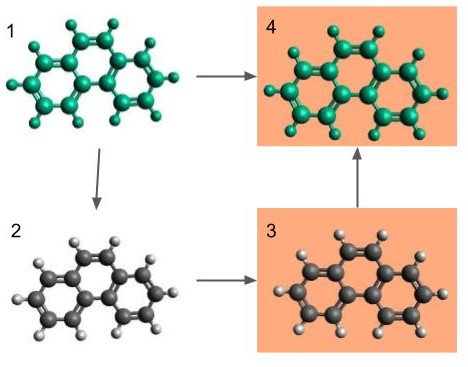
\includegraphics[scale=0.6]{Figures/cicclotermo.jpg}
\caption{Thermodynamic cycle for solvation free energy calculations with molecular dynamics (Adapted from \citeonline{klimovich})}
\label{thermcy}
\end{figure}

The solvation free energy between sates 1 and 2 in the cycle is the one associated with turning off the molecule's non bonded interactions in the gas phase. The following transformation, $\Delta G_{2 \rightarrow 3}$, is the free energy of moving the non-interacting molecule in the gas phase to the solvent and is equal to zero since the transformation of a non interacting molecule doesn't depend on the environment. Lastly, $\Delta G_{3 \rightarrow 4}$ is the free energy required to the  the non-interaction molecule in the aqueous phase regain its non-bonded interactions.  The solvation free energy calculation can be classified according to the types of the non bonded interactions that are turned of in the $1 \rightarrow 2$ and $ 3 \rightarrow 4$ parts of the cycle. If both the non-bonded interactions with the environment and the internal interactions are turned of, this is the annihilation free energy. Meanwhile, if only the non-bonded interactions with the environment are turned off,this is the decoupling free energy. In this later case, $\Delta G_{1 \rightarrow 2} = 0$ and the $\Delta G_{solv} = \Delta G_{3 \rightarrow 4} $. The methods used to carry out theses transformations scale the solute charges to zero and then turn of the interactions corresponding to the Lennard Jones potential. In order to carry out the later process, a modified potential with a coupling parameter $\lambda$ is used. Each $\lambda$ represent an alchemical state and, when $\lambda=0$, there is no interaction with the solvent and, when $\lambda=1$, the interactions are fully activated. The coupling of the $\lambda$ parameter could be linear, but it could generate numerical problems related to the exponential part of the Potential. That's why the non-linear soft-core scheme \cite{beutler1994} is usually used, the so called soft core Lennard-Jones potential is given by:

\begin{equation}
\label{eq:softcore}
\begin{aligned}
U_{LJ}^{sc}(r) {}=& 4\lambda\epsilon \left\lbrace\frac{1}{\left[\alpha(1-\lambda)^{2}+ (r/\sigma)^{6}\right]^{2}} - \frac{1}{\alpha(1-\lambda)^2+(r/\sigma)^{6}}\right\rbrace
\end{aligned}
\end{equation}
where $\alpha$ is a constant in which the value of 0.5 is normally assumed to it. The $\Delta G_{3 \rightarrow 4}$ can be then obtained by doing independent simulations in different values of $\lambda$ or by doing expanded ensemble simulations \cite{lyubartsev} which samples all state in a single simulation. This method allows a faster sampling across the alchemical states considering that the kinetic barriers are not substantial. 

\section{Post simulation methods}

The data obtained with molecular dynamics simulations method explained in the section above contain the potential energies correspondent to each $\lambda$. These potential energies obtained then needs to be post processed and analyzed in order to calculate the solvation free energies. Some of the widely used method for these calculations are going to be briefly describe below. 

\subsection{Thermodynamic integration}

The thermodynamic integration method \cite{kirkwood1935} uses equilibrium averages to evaluate the derivative of the potential energy with respect to the coupling parameter. Then, the free energies are obtained as the integration of the derivatives of the initial and final state:

\begin{equation}
\label{eq:ti}
\begin{aligned}
\Delta G_{solv} = \int_{0}^{1} \frac{\partial U}{\partial \lambda} d\lambda
\end{aligned}
\end{equation}

The integration in Eq. \eqref{eq:ti} is obtained by interpolating the output data form the simulations in different ways. Some examples of methods for the interpolations are the trapezoidal rule or natural cubic spline \cite{bareva}. There are also other more complex schemes that are usually system specific as the works of \citeonline{garrido2010} and \citeonline{shyu2009} and that use fitting functions to interpolate the data. 

\subsection{Free energy of Pertubation (FEP)}

The free energy of perturbation method \cite{zwanzig1954} is the oldest and the of the most general purpose strategy to calculate free energy differences. In this method, the difference between two thermodynamic states A and B is given by:

\begin{equation}
\label{eq:fep}
\begin{aligned}
\Delta F = -\kappa_{b}ln \langle{e^{-\beta (U_{B}-U_{A})}}\rangle_{A}
\end{aligned}
\end{equation}

According to the equation above, the free energy difference is calculated by doing an average over the potential energies of state A and B obtained during the simulation of state A. This method only provides precise free energies when there  is a great overlap between the state that is, the state B represents a small perturbation in state A. 

\subsection{Bennet Acceptance Ratio (BAR)}


 En realidad, cuando se simulan
dos estados existe un método que asegura convergencia en el cálculo de deltaF sin exigir un
solapamiento considerable de las distribuciones configuracionales. En particular, nos estamos
refiriendo al método Bennett Acceptance Ratio [148], que describimos en la próxima sección.

%Recent work \cite{mobley2014,mobley2017} made available a big database of hydration free energy of small molecules using the GAFF force field. A comparision of polar and nonpolar contributions to these hydratation free energy inidcated the significance of each the terms  \cite{izairi2017}. Garrido \textit{et al.} \citep{garrido,garrido2011} calculated the free energy of solvation of large alkanes in 1-octanol and water with three different force fields (TraPPE, Gromos, OPLS-AA/TraPPE) and the solvation free energy of propane and benzene in non aqueous solvents like n-hexadecane, n-hexane, ethyl benzene, acetone  with the force fields TraPPE-UA and TraPPE-AA. Roy \textit{et al.} \citep{roy2017} addressed the choice of the Lennard Jones parameters for predicting solvation free energy in 1-octanol. Gon\c{c}alves and Stassen \citep{goncalves} calculated the free energy of solvation in the solvents tetrachloride, chloroform and benzene with GROMOS force field. Using the GAFF and the polarazible AMOEBA force fields, Mohamed \textit{et al.} \citep{mohamed2016} evaluated the solvation free energy of small molecules in toluene, chloroform and acetonitrile and obtained a mean unsigned error of 1.22 $kcal/mol$ for the AMOEBA and 0.66 $kcal/mol$ for the GAFF. 



benchmark
Specifically, in some
situations, free energy calculations appear to be capable
of achieving RMS errors in the 1-2 kcal/mol range with
current force fields, even in prospective applications.

The most immediate application of these techniques is to guide synthesis for lead optimization, but applications to scaffold
hopping and in other areas also appear possible.

At the same time, it is clear that not all situations are
so favorable, so it is worth asking what level of accuracy
is actually needed

The present review focuses on a class of methods in
which free energy differences are computed with simulations that sample Boltzmann distributions of molecular configurations. These samples are usually generated by molecular dynamics (MD) simulations [92], with
the system effectively coupled to a heat bath at constant temperature, but Monte Carlo methods may also
be used [32, 120, 121]. 

In either case, the energy of a
given configuration is provided by a potential function,
or force field, which estimates the potential energy of
a system of solute and solvent molecules as a function
of the coordinates of all of its atoms.

In
all cases, however, the calculations yield the free energy
difference between two states of a molecular system, and
they do so by computing the reversible work for changing
the initial state to the final one. 
